% =====================================================================
%  SmartDental — Manual de usuario
%  Compilación: pdflatex manual && pdflatex manual
% =====================================================================
\documentclass[11pt]{article}
\usepackage{sd-estilo}
\hypersetup{pdftitle={SmartDental — Manual de usuario},pdfsubject={Manual de usuario},pdfauthor={}}

\begin{document}

\sdportada

\pagenumbering{roman}
\setcounter{page}{2}
{\hypersetup{linkcolor=sdink}\tableofcontents}
\clearpage
\pagenumbering{arabic}

% =====================================================================
\capitulo{Antes de empezar}\label{sec:antes}
% =====================================================================

SmartDental es un sistema web para dirigir un consultorio odontológico desde el navegador: la agenda de cada profesional, el directorio de pacientes, el odontograma con su cotización, el inventario de insumos, la caja, las conversaciones de WhatsApp y un asistente con inteligencia artificial. Este manual explica, pantalla por pantalla, qué hace cada elemento y cómo completar cada tarea.

\subsection{Cómo está organizado este manual}

\begin{itemize}
  \item Los capítulos \ref{sec:primeros} a \ref{sec:cuenta} recorren el \textbf{panel de la clínica} en el orden del menú lateral.
  \item El \cref{sec:plataforma} está dedicado a la \textbf{consola de plataforma}, que solo usa quien administra SmartDental.
  \item El \cref{sec:ejemplo} une todo en un caso real, de la primera llamada del paciente al cobro.
  \item Los capítulos finales reúnen la \textbf{solución de problemas}, las preguntas frecuentes, los atajos de teclado y el glosario.
\end{itemize}

Cada capítulo de un módulo empieza con una franja que indica qué perfiles pueden usarlo, sigue con una captura señalizada y termina con los procedimientos paso a paso.

\subsection{Convenciones y señalización}\label{sec:convenciones}

\begin{table}[H]
\centering\small
\caption{Convenciones usadas en el manual}\label{tab:convenciones}
\begin{tabularx}{\linewidth}{@{}P{4.4cm}L@{}}
\toprule
\textbf{Señal} & \textbf{Significado} \\
\midrule
\marca{1}\ \marca{2}\ \marca{3} & Marcador numerado sobre una captura. El recuadro naranja delimita el elemento y la leyenda que sigue a la imagen explica cada número. \\
\boton{Nueva cita} & Botón, pestaña o casilla que se pulsa en la pantalla, escrito tal como aparece. \\
\tecla{Ctrl}\,+\,\tecla{K} & Combinación de teclas. En Mac, \tecla{Ctrl} se sustituye por \tecla{Cmd}. \\
\ruta{Preferencias\sep Tarifario} & Ruta de navegación: sección del menú lateral y apartado dentro de ella. \\
\campo{Profesional responsable} & Nombre de un campo de un formulario. \\
\estado{sdteal}{Confirmada}\ \estado{sdamber}{Pendiente} & Etiquetas de estado tal como se muestran en la interfaz. \\
\rolsi{Odontólogo}\ \rolver{Recepción}\ \rolno{Recepción} & Acceso completo, solo consulta o sin acceso a un módulo. \\
\bottomrule
\end{tabularx}
\end{table}

Además, el texto se acompaña de cinco tipos de aviso:

\begin{sdnota}
Información complementaria que ayuda a entender el funcionamiento.
\end{sdnota}
\begin{sdconsejo}
Una forma más rápida o más cómoda de hacer la tarea.
\end{sdconsejo}
\begin{sdaviso}
Algo que conviene revisar antes de continuar para evitar errores.
\end{sdaviso}
\begin{sdpermiso}
Diferencias de lo que ve o puede hacer cada perfil.
\end{sdpermiso}
\begin{sdpeligro}
Acciones con efecto inmediato sobre datos de pacientes o del equipo.
\end{sdpeligro}

\begin{sdnota}[Datos de las capturas]
Las imágenes se tomaron de la aplicación en funcionamiento con un lote de datos de demostración. Los nombres, documentos y teléfonos que aparecen son ficticios.
\end{sdnota}

\subsection{Requisitos}

\begin{table}[H]
\centering\small
\caption{Requisitos para usar SmartDental}\label{tab:requisitos}
\begin{tabularx}{\linewidth}{@{}P{3.6cm}L@{}}
\toprule
\textbf{Elemento} & \textbf{Requisito} \\
\midrule
Navegador & Google Chrome, Microsoft Edge, Mozilla Firefox o Safari, en una versión reciente. No se instala nada en el equipo. \\
Pantalla & Computadora o tableta para el trabajo diario (desde 1280 píxeles de ancho se ve el menú completo). En el teléfono el menú se pliega y la agenda pasa a primer plano. \\
Conexión & Internet estable. Las acciones que modifican datos esperan la confirmación del servidor antes de darse por hechas. \\
Cuenta & Un usuario creado por el administrador de la clínica (o, para el administrador, por el de la plataforma). No existe registro libre desde el sitio público. \\
Vista 3D & Aceleración gráfica (WebGL) activada en el navegador, habitual en equipos de los últimos años. \\
\bottomrule
\end{tabularx}
\end{table}

\subsection{Perfiles y permisos}\label{sec:roles}

SmartDental reconoce cuatro perfiles. Cada uno ve en el menú lateral solo las secciones que le corresponden, y la base de datos aplica las mismas reglas: ocultar un botón nunca es la única protección.

\begin{table}[H]
\centering\small
\caption{Matriz de permisos del panel de la clínica}\label{tab:matriz}
\begin{tabularx}{\linewidth}{@{}L C{2.6cm} C{2.6cm} C{2.6cm}@{}}
\toprule
\textbf{Sección} & \textbf{Administración} & \textbf{Odontólogo} & \textbf{Recepción} \\
\midrule
Resumen y Mi espacio      & \faIcon{check} & \faIcon{check} & \faIcon{check} \\
Agenda                    & Toda la clínica & Solo la propia & Toda la clínica \\
Pacientes                 & \faIcon{check} & Asignados & \faIcon{check} \\
Registrar pacientes       & \faIcon{check} & \textcolor{sdmuted}{\faIcon{times}} & \faIcon{check} \\
Odontograma y cotización  & \faIcon{check} & \faIcon{check} & \textcolor{sdmuted}{\faIcon{times}} \\
Tarifario                 & Edita & Consulta & \textcolor{sdmuted}{\faIcon{times}} \\
Inventario                & \faIcon{check} & \textcolor{sdmuted}{\faIcon{times}} & \faIcon{check} \\
Caja e ingresos           & \faIcon{check} & \textcolor{sdmuted}{\faIcon{times}} & \textcolor{sdmuted}{\faIcon{times}} \\
WhatsApp                  & Bandeja y ajustes & Sus conversaciones & Sus conversaciones \\
Equipo y plan, Preferencias & \faIcon{check} & \textcolor{sdmuted}{\faIcon{times}} & \textcolor{sdmuted}{\faIcon{times}} \\
Asistente Denti           & \faIcon{check} & Sobre su agenda & \faIcon{check} \\
Contraseña y acceso       & \faIcon{check} & \faIcon{check} & \faIcon{check} \\
\bottomrule
\end{tabularx}
\end{table}

El cuarto perfil, el \textbf{administrador de plataforma}, no trabaja dentro de una clínica: gestiona el conjunto de clínicas desde la consola descrita en el \cref{sec:plataforma}.

% =====================================================================
\capitulo{Primeros pasos}\label{sec:primeros}
% =====================================================================

\subsection{Iniciar sesión}\label{sec:login}

\acceso{s}{s}{s}

\begin{pantalla}{m01_login}{1440}{Pantalla de inicio de sesión}
  \zona{1}{146}{346}{400}{50}
  \zona{2}{146}{453}{400}{50}
  \zonad{3}{386}{419}{160}{22}
  \zona{4}{146}{525}{252}{24}
  \zona{5}{146}{571}{400}{52}
  \zona{6}{180}{651}{334}{24}
  \zonad{7}{512}{42}{112}{24}
\end{pantalla}

\begin{leyenda}
  \li{1}{Correo electrónico} El correo con el que se creó tu usuario.
  \li{2}{Contraseña} El icono del ojo la muestra u oculta mientras escribes.
  \item[\marca{3}]\textbf{¿Olvidaste tu contraseña?}~Inicia la recuperación por correo.
  \li{4}{Recordar mi correo} Lo deja escrito la próxima vez, solo en ese equipo.
  \li{5}{Iniciar sesión} Valida los datos y abre tu panel.
  \li{6}{Escríbenos por WhatsApp} Contacto para clínicas que aún no tienen cuenta.
  \li{7}{Volver al sitio} Regresa a la página pública.
\end{leyenda}

\begin{pasos}
  \paso Abre la dirección del sistema y pulsa \boton{Ingresar}, o entra directamente en \ruta{/login}.
  \paso Escribe tu correo \marca{1} y tu contraseña \marca{2}.
  \paso Si el equipo es tuyo, marca \campo{Recordar mi correo en este equipo} \marca{4}.
  \paso Pulsa \boton{Iniciar sesión} \marca{5}.
\end{pasos}
\resultado{El sistema reconoce tu perfil y abre el panel de tu clínica o la consola de plataforma.}

\begin{sdaviso}[Primer ingreso]
Si tu cuenta se creó con una contraseña temporal, cámbiala en cuanto entres desde \ruta{Contraseña y acceso} (\cref{sec:cuenta}).
\end{sdaviso}

\paragraph{Recuperar la contraseña.} Pulsa \textit{¿Olvidaste tu contraseña?} \marca{3}, escribe tu correo y confirma. Abre el enlace que recibirás, escribe la nueva contraseña dos veces y guárdala; después inicia sesión con normalidad.

\paragraph{Cerrar sesión.} Pulsa \boton{Cerrar sesión} al pie del menú lateral. En un equipo compartido, ciérrala siempre al terminar.

\needspace{0.55\textheight}
\subsection{Recorrido por la interfaz}\label{sec:interfaz}

Todas las secciones del panel comparten la misma estructura. Conocerla una vez basta para moverse por todo el sistema.

\begin{pantalla}{m02_resumen}{1440}{Estructura del panel de la clínica}
  \zona{1}{18}{88}{201}{70}
  \zona{2}{14}{180}{222}{620}
  \zona{3}{276}{16}{190}{50}
  \zona{4}{1037}{23}{155}{40}
  \zonad{5}{1318}{24}{88}{38}
  \zona{6}{318}{344}{412}{46}
  \zona{7}{288}{446}{1110}{178}
  \zona{8}{288}{648}{1110}{252}
  \zonad{9}{1222}{826}{190}{52}
\end{pantalla}

\begin{leyenda}
  \li{1}{Tarjeta de la clínica} Nombre del consultorio y plan contratado.
  \li{2}{Menú lateral} Secciones agrupadas en \emph{Tu consultorio}, \emph{Organización}, \emph{Administración} y \emph{Tu cuenta}. Un resaltado marca la sección activa.
  \li{3}{Ruta y título} Indican dónde estás.
  \li{4}{Búsqueda rápida} Abre el buscador universal (\cref{sec:busqueda}).
  \li{5}{Notificaciones y tema} La campana muestra avisos; la luna o el sol cambia entre tema claro y oscuro.
  \li{6}{Accesos directos} Atajos a las tareas más frecuentes.
  \li{7}{Indicadores} Cifras clave del consultorio.
  \li{8}{Contenido de la sección} El área de trabajo propiamente dicha.
  \li{9}{Denti} Botón flotante del asistente (\cref{sec:denti}).
\end{leyenda}

\needspace{0.55\textheight}
\subsection{Búsqueda rápida}\label{sec:busqueda}

\begin{pantalla}[0.62\linewidth]{m16_paleta}{640}{Búsqueda rápida}
  \zona{1}{18}{12}{556}{34}
  \zonad{2}{586}{16}{38}{24}
  \zona{3}{9}{91}{614}{57}
  \zona{4}{15}{526}{322}{24}
\end{pantalla}

\begin{leyenda}
  \li{1}{Campo de búsqueda} Acepta secciones, acciones y, en el panel de la clínica, el nombre o DNI de un paciente.
  \li{2}{Esc} Cierra el buscador sin hacer nada.
  \li{3}{Resultado activo} Se abre con \tecla{Enter}.
  \li{4}{Ayuda de teclado} Recuerda las teclas disponibles.
\end{leyenda}

Ábrela con \tecla{Ctrl}\,+\,\tecla{K} o con el botón \boton{Buscar} de la cabecera. Muévete con \tecla{$\uparrow$}\,\tecla{$\downarrow$}, abre con \tecla{Enter} y cierra con \tecla{Esc}. Además de ir a cualquier sección, ofrece acciones directas: \textit{Nueva cita}, \textit{Nuevo paciente}, \textit{Preguntarle a Denti} o \textit{Activar tema oscuro}.

\begin{sdconsejo}
Con la búsqueda rápida casi no hace falta usar el ratón: \tecla{Ctrl}\,+\,\tecla{K}, escribe «valeria» y pulsa \tecla{Enter} para abrir la ficha de la paciente.
\end{sdconsejo}

\subsection{Tema claro u oscuro}

El botón de la luna \marca{5} de la cabecera alterna entre los dos temas con una transición suave. La preferencia se guarda en el navegador. Si el sistema operativo tiene activada la opción de reducir el movimiento, la transición se omite.

\needspace{0.55\textheight}
\subsection{Uso en el teléfono}

\begin{figure}[H]
\centering
\begin{minipage}[c]{0.36\linewidth}\centering
\begin{tikzpicture}
  \sbox\sdimgbox{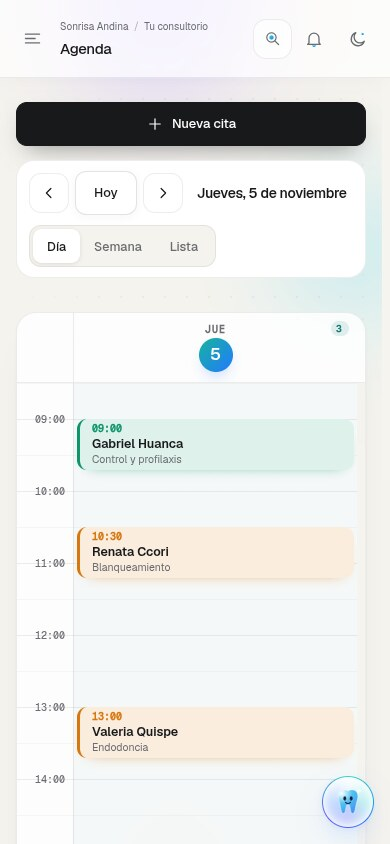
\includegraphics[width=\linewidth]{capturas/m18_movil}}%
  \pgfmathsetmacro\sdpx{\wd\sdimgbox/390}%
  \begin{scope}[x=\sdpx pt,y=-\sdpx pt]
  \node[anchor=north west,inner sep=0pt] (img) at (0,0) {\usebox\sdimgbox};
  \zona{1}{16}{24}{34}{30}
  \zonad{2}{254}{20}{38}{38}
  \zona{3}{16}{102}{350}{44}
  \zona{4}{29}{173}{155}{42}
  \zona{5}{29}{226}{186}{40}
  \zonad{6}{322}{778}{52}{52}
  \draw[sdline,line width=0.7pt,rounded corners=3pt] (img.south west) rectangle (img.north east);
  \end{scope}
\end{tikzpicture}
\end{minipage}\hfill
\begin{minipage}[c]{0.58\linewidth}
\small
\begin{list}{}{\leftmargin=2em\labelwidth=1.5em\labelsep=0.5em\itemsep=0.45em}
  \li{1}{Menú} Despliega el menú lateral sobre la pantalla.
  \li{2}{Buscar} Abre la búsqueda rápida.
  \li{3}{Nueva cita} Siempre a mano, en la parte superior.
  \li{4}{Navegación} Día anterior, hoy y día siguiente.
  \li{5}{Vista} Día, semana o lista.
  \li{6}{Denti} El asistente, en la esquina inferior.
\end{list}
\end{minipage}
\caption{La agenda en un teléfono}\label{fig:m18_movil}
\end{figure}

En pantallas pequeñas la agenda aparece primero y el calendario mensual se desplaza debajo, para que lo urgente quede a la vista.

% =====================================================================
\capitulo{Resumen y Mi espacio}\label{sec:resumen}
% =====================================================================

\acceso{s}{s}{s}

\subsection{Resumen}

Es la portada del consultorio (\cref{fig:m02_resumen}). Saluda según la hora del día y muestra el número de pacientes registrados, las citas con su desglose de pendientes y atendidas, los ingresos registrados y las fichas más recientes. \boton{Ver todos} abre el directorio completo.

\begin{sdpermiso}
Los ingresos solo se muestran a la administración de la clínica.
\end{sdpermiso}

\needspace{0.55\textheight}
\subsection{Mi espacio}\label{sec:espacio}

Mi espacio reúne el trabajo del día de cada persona y es el lugar donde se \textbf{revisan y confirman} los cambios importantes: nada se modifica en bloque sin que antes veas exactamente a quién afecta.

\begin{pantalla}{m03_espacio}{1440}{Mi espacio: agenda autorizada y asistente}
  \zona{1}{303}{338}{506}{70}
  \zonad{2}{709}{281}{100}{42}
  \zona{3}{300}{425}{503}{440}
  \zonad{4}{1215}{177}{182}{40}
  \zona{5}{871}{516}{506}{156}
  \zona{6}{867}{751}{515}{68}
\end{pantalla}

\begin{leyenda}
  \li{1}{Desde y Hasta} Periodo de citas que quieres revisar.
  \li{2}{Actualizar} Vuelve a consultar el servidor.
  \li{3}{Citas autorizadas} Solo las que tu perfil puede ver; las casillas permiten seleccionar varias.
  \li{4}{Atender conversaciones} Acceso directo a WhatsApp.
  \li{5}{Preguntas sugeridas} Un clic las envía a Denti.
  \li{6}{Instrucción para Denti} Escribe tu consulta con tus palabras.
\end{leyenda}

\begin{pasos}
  \paso Ajusta el periodo \marca{1} y pulsa \boton{Actualizar} \marca{2}.
  \paso Marca las citas sobre las que quieras actuar \marca{3}. Aparece un panel con las operaciones disponibles para la selección, como confirmarlas o proponer un nuevo horario.
  \paso Revisa el resumen que muestra el sistema: qué citas cambiarán y si se notificará al paciente.
  \paso Confirma. El resultado de cada cita se muestra por separado; si alguna no pudo cambiarse, se explica el motivo.
\end{pasos}

% =====================================================================
\capitulo{Agenda}\label{sec:agenda}
% =====================================================================

\acceso{s}{s}{s}

\begin{pantalla}{m04_agenda}{1440}{Agenda semanal}
  \zona{1}{282}{120}{264}{42}
  \zona{2}{284}{178}{262}{290}
  \zona{3}{282}{483}{264}{163}
  \zona{4}{577}{131}{320}{42}
  \zonad{5}{1199}{131}{186}{42}
  \zona{6}{952}{224}{108}{62}
  \zona{7}{954}{360}{104}{52}
  \zonad{8}{844}{360}{102}{52}
\end{pantalla}

\begin{leyenda}
  \li{1}{Nueva cita} Abre la reserva guiada.
  \li{2}{Calendario del mes} Los días con citas llevan una marca; un clic salta a ese día.
  \li{3}{Resumen del periodo} Citas activas, pendientes, confirmadas y canceladas de lo que estás viendo.
  \li{4}{Navegación} Periodo anterior, \boton{Hoy} y periodo siguiente.
  \li{5}{Vista} \boton{Día}, \boton{Semana} o \boton{Lista}.
  \li{6}{Cabecera del día} Número de citas del día; el día actual va resaltado.
  \li{7}{Tarjeta de cita} Hora, paciente y motivo, con el color de su estado.
  \li{8}{Citas superpuestas} El indicador «+N» agrupa las que coinciden en la misma hora; púlsalo para ver la lista completa.
\end{leyenda}

\subsection{Estados de una cita}

\begin{table}[H]
\centering\small
\caption{Estados de una cita}\label{tab:estados}
\begin{tabularx}{\linewidth}{@{}P{3.2cm}L@{}}
\toprule
\textbf{Estado} & \textbf{Significado} \\
\midrule
\estado{sdamber}{Pendiente} & Reservada, a la espera de que el paciente confirme. Tarjeta en tono ámbar. \\
\estado{sdteal}{Confirmada} & El paciente confirmó su asistencia. Tarjeta en tono verde azulado. \\
\estado{sdmuted}{Cancelada} & No se realizará; el horario vuelve a quedar libre para otra reserva. \\
\bottomrule
\end{tabularx}
\end{table}

\needspace{0.55\textheight}
\subsection{Reservar una cita}\label{sec:reservar}

\begin{figure}[H]
\centering
\begin{minipage}[c]{0.46\linewidth}\centering
\begin{tikzpicture}
  \sbox\sdimgbox{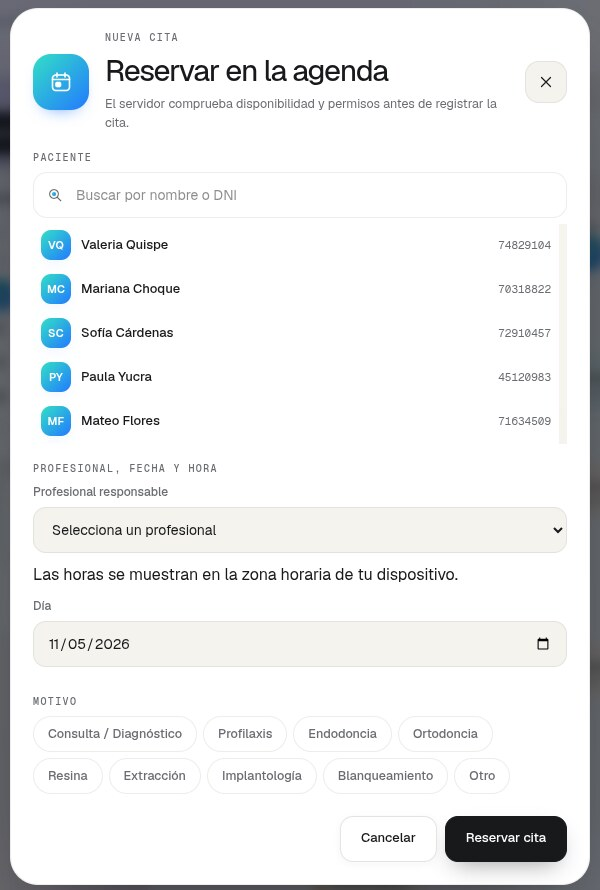
\includegraphics[width=\linewidth]{capturas/m05_nueva_cita}}%
  \pgfmathsetmacro\sdpx{\wd\sdimgbox/600}%
  \begin{scope}[x=\sdpx pt,y=-\sdpx pt]
  \node[anchor=north west,inner sep=0pt] (img) at (0,0) {\usebox\sdimgbox};
  \zona{1}{33}{172}{534}{46}
  \zona{2}{33}{224}{530}{220}
  \zona{3}{33}{507}{534}{46}
  \zona{4}{33}{621}{534}{46}
  \zona{5}{33}{716}{480}{78}
  \zonad{6}{445}{816}{122}{46}
  \draw[sdline,line width=0.7pt,rounded corners=3pt] (img.south west) rectangle (img.north east);
  \end{scope}
\end{tikzpicture}
\end{minipage}\hfill
\begin{minipage}[c]{0.5\linewidth}
\small
\begin{list}{}{\leftmargin=2em\labelwidth=1.5em\labelsep=0.5em\itemsep=0.5em}
  \li{1}{Buscar paciente} Por nombre o DNI.
  \li{2}{Resultados} Un clic selecciona al paciente.
  \li{3}{Profesional responsable} Al elegirlo, el sistema consulta su disponibilidad real.
  \li{4}{Día} Fecha de la cita; debajo aparecen los horarios libres.
  \li{5}{Motivo} Opciones frecuentes u \boton{Otro} para escribirlo.
  \li{6}{Reservar cita} Registra la cita tras validarla en el servidor.
\end{list}
\end{minipage}
\caption{Reserva de una nueva cita}\label{fig:m05_nueva_cita}
\end{figure}

\begin{pasos}
  \paso Pulsa \boton{Nueva cita}.
  \paso Busca al paciente \marca{1} y selecciónalo en la lista \marca{2}.
  \paso Elige al \campo{Profesional responsable} \marca{3} y el \campo{Día} \marca{4}. Mientras aparece \textit{Consultando disponibilidad real…}, el sistema cruza el horario del profesional con sus citas.
  \paso Elige uno de los horarios libres y el \campo{Motivo} \marca{5}.
  \paso Pulsa \boton{Reservar cita} \marca{6}.
\end{pasos}
\resultado{Aparece el aviso «Cita registrada» y la tarjeta se muestra en la agenda como pendiente.}

\begin{sdnota}
Las horas se muestran en la zona horaria de tu dispositivo. Si eliges un horario que ya pasó, el sistema lo indica con «Horario pasado» y no reserva.
\end{sdnota}

\subsection{Confirmar, cancelar o atender una cita}

Haz clic sobre una tarjeta para abrir su detalle: fecha, hora, paciente, motivo, estado y DNI. Desde ahí:

\begin{itemize}
  \item \boton{Revisar en Mi espacio} lleva la confirmación a Mi espacio, donde se revisa antes de aplicarse (\cref{sec:espacio}).
  \item \boton{Cancelar cita} abre la ventana \textit{Revisar cancelación}, que muestra lo que cambiará; la cita solo se cancela al confirmar.
  \item \boton{Atender desde la clínica} abre las conversaciones de WhatsApp.
  \item \boton{Ver ficha} abre la ficha clínica del paciente.
\end{itemize}

\begin{sdpermiso}
Un odontólogo solo ve su propia agenda. La administración y la recepción ven la de todos los profesionales.
\end{sdpermiso}

% =====================================================================
\capitulo{Pacientes}\label{sec:pacientes}
% =====================================================================

\acceso{s}{s}{s}

\begin{pantalla}{m06_pacientes}{1440}{Directorio clínico}
  \zonad{1}{1239}{177}{159}{42}
  \zona{2}{282}{260}{1116}{46}
  \zona{3}{282}{318}{872}{38}
  \zonad{4}{1164}{317}{78}{40}
  \zona{5}{282}{404}{364}{133}
  \zonad{6}{579}{420}{52}{60}
  \zonad{7}{578}{489}{34}{32}
\end{pantalla}

\begin{leyenda}
  \li{1}{Nuevo paciente} Abre el formulario de registro.
  \li{2}{Buscador} Filtra al escribir por nombre, DNI, teléfono o correo.
  \li{3}{Filtro por tratamiento} Muestra solo a quienes siguen un tratamiento.
  \li{4}{Vista} Tarjetas o lista.
  \li{5}{Tarjeta del paciente} Iniciales, nombre, DNI y teléfono.
  \li{6}{Índice CPO-D} Calculado a partir de su odontograma.
  \li{7}{Abrir ficha} Abre la ficha clínica.
\end{leyenda}

\subsection{Registrar un paciente}

\begin{pasos}
  \paso Pulsa \boton{Nuevo paciente} \marca{1}.
  \paso Completa los campos obligatorios, marcados con *: \campo{Nombre completo} y \campo{Teléfono}.
  \paso Añade, si los conoces, el \campo{DNI}, el \campo{Correo}, el \campo{Tratamiento} y las \campo{Alergias conocidas} (por ejemplo, «Penicilina» o «Ninguna»).
  \paso Pulsa \boton{Registrar paciente}.
\end{pasos}
\resultado{Aparece el aviso «Paciente registrado» y la tarjeta se suma al directorio.}

\begin{sdpermiso}
Registran pacientes la administración y la recepción. Un odontólogo ve a los pacientes que tiene asignados.
\end{sdpermiso}

\needspace{0.55\textheight}
\subsection{La ficha clínica}

\begin{pantalla}{m06b_ficha}{1148}{Ficha clínica de un paciente}
  \zona{1}{95}{20}{330}{86}
  \zona{2}{23}{121}{277}{48}
  \zona{3}{23}{224}{1102}{70}
  \zona{4}{23}{304}{546}{91}
  \zona{5}{23}{413}{525}{44}
  \zonad{6}{1083}{43}{42}{42}
\end{pantalla}

\begin{leyenda}
  \li{1}{Identificación} Nombre, DNI y fecha de registro.
  \li{2}{Pestañas} \boton{Datos}, \boton{Odontograma} y \boton{Citas}.
  \li{3}{Datos de contacto} Teléfono, correo, tratamiento y alergias. Una alergia registrada se destaca en color.
  \li{4}{Resumen clínico} Piezas registradas en el odontograma y el índice CPO-D con su desglose.
  \li{5}{Acciones} Conversaciones, \boton{Agendar cita} y \boton{Editar datos}.
  \li{6}{Cerrar} Vuelve al directorio.
\end{leyenda}

\begin{sdnota}
La ficha respeta el ámbito de atención: los registros de cada profesional se conservan por separado y solo se muestran a quien tiene permiso para verlos.
\end{sdnota}

% =====================================================================
\capitulo{Odontograma}\label{sec:odontograma}
% =====================================================================

\acceso{s}{s}{n}

El odontograma registra el estado de cada pieza con la convención clínica de colores: \textcolor{sdred}{\textbf{rojo}} para los hallazgos o piezas en mal estado y \textcolor{sdblue}{\textbf{azul}} para los tratamientos realizados o en buen estado.

\begin{pantalla}{m07_odontograma}{1440}{Odontograma de una paciente}
  \zona{1}{283}{120}{258}{718}
  \zona{2}{561}{97}{837}{116}
  \zona{3}{571}{240}{816}{92}
  \zona{4}{571}{341}{220}{42}
  \zonad{5}{803}{341}{82}{42}
  \zona{6}{577}{428}{205}{40}
  \zonad{7}{817}{428}{248}{40}
  \zona{8}{577}{482}{488}{214}
  \zonad{9}{1099}{411}{298}{223}
  \zona{10}{561}{783}{220}{117}
  \zona{11}{799}{783}{332}{117}
  \zonad{12}{1149}{783}{60}{30}
\end{pantalla}

\begin{leyenda}
  \li{1}{Pacientes} Buscador y lista; el paciente activo queda resaltado.
  \li{2}{Paciente} Nombre y DNI del odontograma abierto.
  \li{3}{Herramientas} Hallazgos y tratamientos, con el número de marcas de cada uno.
  \li{4}{Estado} \boton{Mal estado} (rojo) o \boton{Buen estado} (azul).
  \li{5}{Deshacer y rehacer} También con el teclado.
  \li{6}{Vista} \boton{Odontograma} 2D o \boton{Arcada 3D}.
  \li{7}{Dentición} \boton{Permanente}, \boton{Temporal} o \boton{Mixta}.
  \li{8}{Diagrama} Cada pieza con sus cinco caras y su número FDI.
  \li{9}{Detalle de la pieza} Marcas, nota y acciones de la pieza elegida.
  \li{10}{Índice CPO-D} Cariadas, perdidas, obturadas y total.
  \li{11}{Observaciones generales} Diagnóstico y plan de tratamiento.
  \li{12}{Historial} Versiones guardadas, con fecha y autor.
\end{leyenda}

\subsection{Notación FDI y caras de la pieza}

Cada pieza se identifica con dos dígitos: el primero es el \textbf{cuadrante} y el segundo la \textbf{posición}, contada desde la línea media. El diagrama se dibuja como si se mirara al paciente de frente: su derecha queda a la izquierda de la pantalla.

\begin{figure}[H]
\centering
\begin{tikzpicture}[x=0.78cm,y=0.78cm,font=\sffamily\scriptsize]
  \foreach \i in {1,...,8}{
    \node[draw=sdline,fill=sdsoft,rounded corners=2pt,minimum size=0.62cm] at (-\i+0.5,1) {1\i};
    \node[draw=sdline,fill=sdsoft,rounded corners=2pt,minimum size=0.62cm] at (\i-0.5,1) {2\i};
    \node[draw=sdline,fill=sdsoft,rounded corners=2pt,minimum size=0.62cm] at (-\i+0.5,-0.1) {4\i};
    \node[draw=sdline,fill=sdsoft,rounded corners=2pt,minimum size=0.62cm] at (\i-0.5,-0.1) {3\i};
  }
  \draw[sdteal,line width=0.9pt,dashed] (0,-0.75) -- (0,1.65);
  \draw[sdteal,line width=0.9pt,dashed] (-8.3,0.45) -- (8.3,0.45);
  \node[text=sdteal,font=\sffamily\bfseries\scriptsize] at (-4,1.95) {Cuadrante 1 · superior derecho};
  \node[text=sdteal,font=\sffamily\bfseries\scriptsize] at (4,1.95) {Cuadrante 2 · superior izquierdo};
  \node[text=sdteal,font=\sffamily\bfseries\scriptsize] at (-4,-1.05) {Cuadrante 4 · inferior derecho};
  \node[text=sdteal,font=\sffamily\bfseries\scriptsize] at (4,-1.05) {Cuadrante 3 · inferior izquierdo};
  \node[text=sdmuted] at (0,-1.6) {Dentición temporal: cuadrantes 5 a 8, cinco piezas por cuadrante (55 a 51, 61 a 65, 71 a 75, 85 a 81)};
  % Caras
  \begin{scope}[shift={(10.6,0.45)},x=1cm,y=1cm]
    \draw[sdink,line width=0.8pt] (0,0) circle (0.95);
    \draw[sdink,line width=0.8pt] (0,0) circle (0.38);
    \foreach \a in {45,135,225,315}{\draw[sdink,line width=0.8pt] (\a:0.38) -- (\a:0.95);}
    \fill[sdred!80] (0,0) circle (0.36);
    \node[font=\sffamily\bfseries\scriptsize,text=white] at (0,0) {O};
    \node at (0,0.67) {V}; \node at (0,-0.67) {L}; \node at (-0.67,0) {M}; \node at (0.67,0) {D};
    \node[text=sdmuted,align=center,font=\sffamily\tiny] at (0,-1.35) {Caras de una pieza\\(caries oclusal en rojo)};
  \end{scope}
\end{tikzpicture}
\caption{Numeración FDI de la dentición permanente y caras de una pieza}\label{fig:fdi}
\end{figure}

Las caras son \textbf{V} vestibular, \textbf{M} mesial, \textbf{O} oclusal, \textbf{D} distal y \textbf{L} lingual (palatina en el maxilar superior). Las piezas 18, 28, 38 y 48 son los terceros molares.

\subsection{Herramientas}

\begin{table}[H]
\centering\small
\caption{Herramientas del odontograma y su atajo de teclado}\label{tab:herramientas}
\begin{tabularx}{\linewidth}{@{}C{1.2cm}P{3.6cm}P{2.2cm}L@{}}
\toprule
\textbf{Tecla} & \textbf{Herramienta} & \textbf{Se marca en} & \textbf{Uso habitual} \\
\midrule
\tecla{1} & Caries & Cara & Lesión cariosa en una superficie (rojo). \\
\tecla{2} & Restauración & Cara & Resina u obturación existente (azul) o a cambiar (rojo). \\
\tecla{3} & Sellante & Cara & Sellante de fosas y fisuras. \\
\tecla{4} & Corona & Pieza & Corona completa existente o indicada. \\
\tecla{5} & Endodoncia & Pieza & Tratamiento de conductos realizado o indicado. \\
\tecla{6} & Implante & Pieza & Implante dental. \\
\tecla{7} & Fractura & Pieza & Fractura coronaria (rojo). \\
\tecla{8} & Extracción indicada & Pieza & Pieza a extraer (rojo). \\
\tecla{9} & Ausente & Pieza & Pieza que ya no está en boca. \\
\tecla{0} & Borrar & Cara o pieza & Quita la marca que se toque. \\
\bottomrule
\end{tabularx}
\end{table}

\subsection{Registrar hallazgos y tratamientos}

\begin{pasos}
  \paso Elige al paciente en la lista \marca{1} o ábrelo desde su ficha.
  \paso Comprueba la \campo{Dentición} \marca{7}: permanente, temporal o mixta.
  \paso Elige una herramienta \marca{3} (o pulsa su tecla) y el estado \marca{4}.
  \paso Toca la cara de la pieza o la pieza completa en el diagrama \marca{8}. Vuelve a tocarla para quitar la marca.
  \paso Si hace falta, escribe una nota en el detalle de la pieza \marca{9} y las \campo{Observaciones generales} \marca{11}.
  \paso Pulsa \boton{Guardar odontograma}. Mientras haya cambios sin guardar, un aviso lo recuerda.
\end{pasos}
\resultado{Se crea una versión en el historial y el índice CPO-D se actualiza al momento.}

\begin{sdconsejo}
Con una pieza seleccionada, \tecla{$\leftarrow$} y \tecla{$\rightarrow$} recorren las piezas vecinas. Combinado con las teclas \tecla{1}–\tecla{9}, se registra un examen completo sin usar el ratón.
\end{sdconsejo}

\needspace{0.55\textheight}
\subsection{Arcada 3D}

\begin{pantalla}{m08_odo3d}{1440}{Arcada 3D coloreada por estado}
  \zona{1}{577}{428}{205}{40}
  \zonad{2}{917}{428}{148}{40}
  \pin{3}{672}{624}
  \pin{4}{972}{624}
  \pin{5}{668}{653}
  \zona{6}{577}{482}{488}{418}
\end{pantalla}

\begin{leyenda}
  \li{1}{Arcada 3D} Cambia de la vista 2D a la tridimensional.
  \li{2}{Encuadre} Vista \boton{Oclusal} (desde arriba) o \boton{Frontal}.
  \li{3}{Pieza con hallazgo} Su número va sobre fondo rojo.
  \li{4}{Pieza tratada} Número sobre fondo azul.
  \li{5}{Pieza sin marcas} Número neutro.
  \li{6}{Modelo} Arrastra para girarlo; toca una pieza para ver su detalle.
\end{leyenda}

\begin{sdnota}
La vista 3D refleja exactamente el mismo registro que el diagrama 2D: no es un dato aparte. Las piezas ausentes se muestran translúcidas.
\end{sdnota}

\subsection{Índices CPO-D y ceo-d}

El sistema calcula los índices epidemiológicos sin intervención del usuario:

\[
\text{CPO-D} = C + P + O \qquad\qquad \text{ceo-d} = c + e + o
\]

donde $C$ son las piezas permanentes cariadas, $P$ las perdidas (ausentes o con extracción indicada) y $O$ las obturadas; en dentición temporal, $c$, $e$ y $o$ son las cariadas, con extracción indicada y obturadas. En la paciente de la \cref{fig:m07_odontograma}, $3 + 2 + 3 = 8$. En dentición \textbf{mixta} se muestran ambos índices por separado.

\subsection{Imprimir}

\boton{Imprimir odontograma} genera una versión limpia para papel o PDF, con el nombre del paciente, la fecha, el diagrama, la leyenda de colores y las observaciones, sin menús ni botones.

% =====================================================================
\capitulo{Cotización y tarifario}\label{sec:cotizacion}
% =====================================================================

\acceso{s}{s}{n}

Debajo del odontograma se encuentra la \textbf{Cotización del tratamiento}. Se calcula sola a partir de las marcas en rojo con el tarifario de la clínica; las marcas azules son tratamientos ya realizados y no se cobran.

\begin{pantalla}{m09_cotizacion}{1440}{Cotización calculada desde el odontograma}
  \zona{1}{579}{112}{520}{100}
  \zona{2}{579}{222}{345}{42}
  \zona{3}{579}{280}{402}{380}
  \zona{4}{579}{668}{374}{198}
  \zona{5}{1003}{285}{375}{385}
  \zonad{6}{1290}{708}{74}{32}
  \zona{7}{1008}{755}{360}{34}
  \zona{8}{1008}{796}{200}{24}
\end{pantalla}

\begin{leyenda}
  \li{1}{Total aproximado} Y cuántas piezas con hallazgos se consideraron.
  \li{2}{Acciones} \boton{Tarifario}, \boton{Imprimir} y \boton{Guardar cotización}.
  \li{3}{Tratamientos sugeridos} Uno por hallazgo, con la pieza y el motivo; desmarca los que no se harán.
  \li{4}{Añadir al presupuesto} Consulta, profilaxis, procedimientos propios e implantes.
  \li{5}{Detalle} Procedimientos agrupados con cantidad y precio editable.
  \li{6}{Descuento} En porcentaje.
  \li{7}{Total} Se recalcula con cada cambio.
  \li{8}{Nota para el paciente} Sesiones, controles incluidos o indicaciones.
\end{leyenda}

\subsection{De hallazgo a procedimiento}

\begin{table}[H]
\centering\small
\caption{Reglas de la cotización automática (precios referenciales en soles)}\label{tab:reglas}
\begin{tabularx}{\linewidth}{@{}P{4.2cm}L r@{}}
\toprule
\textbf{Hallazgo en rojo} & \textbf{Procedimiento sugerido} & \textbf{S/} \\
\midrule
Caries en una cara & Restauración con resina & 80 \\
Cada cara cariada adicional & Cara adicional de resina & 30 \\
Restauración en mal estado & Cambio de restauración & 90 \\
Sellante en mal estado & Sellante de fosas y fisuras & 40 \\
Fractura & Reconstrucción coronaria & 150 \\
Corona en mal estado & Corona metal-porcelana & 650 \\
Endodoncia indicada & Endodoncia anterior, premolar o molar, según la pieza & 350 / 450 / 600 \\
Implante en mal estado & Tratamiento periimplantario & 200 \\
Extracción indicada & Extracción simple; de tercer molar en 18, 28, 38 y 48 & 80 / 250 \\
Pieza ausente & Implante dental, solo si se elige reponerla & 3500 \\
\bottomrule
\end{tabularx}
\end{table}

\paragraph{Ejemplo.} La pieza 16 tiene caries en las caras oclusal y mesial: se sugiere una restauración con resina (S/~80) más una cara adicional (S/~30), en total S/~110. Si la pieza ya tiene una corona en mal estado, las caries de esa pieza no se cobran por separado porque la corona las resuelve.

\subsection{Preparar y entregar la cotización}

\begin{pasos}
  \paso Registra los hallazgos en el odontograma (\cref{sec:odontograma}).
  \paso Revisa los tratamientos sugeridos \marca{3} y desmarca los que el paciente no hará ahora.
  \paso Añade lo que corresponda en \textit{Añadir al presupuesto} \marca{4}.
  \paso Ajusta un precio puntual en el detalle \marca{5} o aplica un descuento \marca{6}.
  \paso Escribe una \campo{Nota para el paciente} \marca{8}.
  \paso Pulsa \boton{Imprimir} para entregarla en papel o PDF, y \boton{Guardar cotización} para dejar una copia en la ficha.
\end{pasos}
\resultado{La ficha conserva las diez cotizaciones más recientes del paciente.}

\begin{sdaviso}
Toda cotización es aproximada: el plan definitivo depende de la evaluación clínica. Así lo indica también el documento impreso.
\end{sdaviso}

\needspace{0.55\textheight}
\subsection{Tarifario de la clínica}\label{sec:tarifario}

\acceso{s}{v}{n}

\begin{pantalla}{m14_tarifario}{1440}{Tarifario en Preferencias}
  \zona{1}{303}{207}{340}{40}
  \zona{2}{948}{208}{276}{38}
  \zonad{3}{1229}{208}{148}{38}
  \zona{4}{303}{262}{1074}{38}
  \zona{5}{303}{314}{350}{212}
  \zonad{6}{521}{360}{113}{36}
  \zona{7}{303}{826}{1074}{74}
\end{pantalla}

\begin{leyenda}
  \li{1}{Buscar procedimiento} Filtra la lista al escribir.
  \li{2}{Ajustar todo} Sube o baja todos los precios en un porcentaje.
  \li{3}{Precios referenciales} Restablece los valores de partida.
  \li{4}{Ejemplo vivo} Muestra cómo se cotiza una caries de dos caras con tus precios.
  \li{5}{Especialidad} Procedimientos agrupados por área clínica.
  \li{6}{Precio} Se edita directamente en soles.
  \li{7}{Procedimientos de la clínica} Lo que ofreces y no sale del odontograma.
\end{leyenda}

\begin{pasos}
  \paso Entra en \ruta{Preferencias\sep Tarifario} o pulsa \boton{Tarifario} en una cotización.
  \paso Cambia los precios que necesites \marca{6}. Para un ajuste general, escribe el porcentaje en \campo{Ajustar todo} y pulsa \boton{Subir} o \boton{Bajar} \marca{2}; los precios se redondean a múltiplos de S/~5.
  \paso En \textit{Procedimientos de la clínica} \marca{7} añade, por ejemplo, «Blanqueamiento dental» con su precio. Las filas vacías se ignoran.
  \paso Pulsa \boton{Guardar}. Los nuevos precios se aplican a las cotizaciones siguientes.
\end{pasos}

\begin{sdpermiso}
Solo la administración modifica el tarifario. Los odontólogos lo consultan desde la cotización.
\end{sdpermiso}

% =====================================================================
\capitulo{Inventario}\label{sec:inventario}
% =====================================================================

\acceso{s}{n}{s}

\begin{pantalla}{m10_inventario}{1440}{Inventario con alertas de reposición}
  \zonad{1}{1248}{177}{150}{42}
  \zona{2}{282}{260}{1116}{101}
  \zona{3}{282}{380}{1116}{130}
  \zona{4}{282}{528}{1116}{46}
  \zona{5}{282}{620}{270}{225}
  \zona{6}{299}{716}{236}{20}
  \zona{7}{299}{785}{236}{44}
  \zonad{8}{498}{750}{38}{20}
\end{pantalla}

\begin{leyenda}
  \li{1}{Nuevo insumo} Registra un material.
  \li{2}{Indicadores} Total de insumos, agotados, bajo mínimo y en stock.
  \li{3}{Requieren reposición} Ordenados del más urgente al menos urgente, con acceso directo a \boton{Reponer}.
  \li{4}{Buscar insumo} Filtra por nombre.
  \li{5}{Tarjeta del insumo} Unidades disponibles y estado.
  \li{6}{Barra de nivel} La marca vertical señala el stock mínimo.
  \li{7}{Movimientos} \boton{$-$ Salida} y \boton{+ Reponer}.
  \li{8}{Editar} Cambia el nombre o el stock mínimo.
\end{leyenda}

\begin{table}[H]
\centering\small
\caption{Semáforo de stock}\label{tab:semaforo}
\begin{tabularx}{\linewidth}{@{}P{3cm}L@{}}
\toprule
\textbf{Estado} & \textbf{Condición} \\
\midrule
\estado{sdred}{Agotado} & No quedan unidades. \\
\estado{sdamber}{Bajo mínimo} & Quedan unidades, pero igual o menos que el stock mínimo. \\
\estado{sdteal}{En stock} & La cantidad supera el stock mínimo. \\
\bottomrule
\end{tabularx}
\end{table}

\begin{pasos}
  \paso Para registrar un insumo, pulsa \boton{Nuevo insumo} \marca{1}, escribe el \campo{Nombre del insumo}, la \campo{Cantidad inicial} y el \campo{Stock mínimo}, y guarda.
  \paso Para registrar un consumo, pulsa \boton{$-$ Salida} \marca{7}, indica las unidades con los botones $-$ y $+$ y confirma. El sistema muestra cuántas \textit{Quedarán} antes de guardar e impide sacar más de las disponibles.
  \paso Para una compra, pulsa \boton{+ Reponer}: el sistema propone la cantidad necesaria para duplicar el mínimo.
\end{pasos}
\resultado{El aviso confirma el cambio, por ejemplo «Guantes de nitrilo: 3 $\rightarrow$ 10 unidades».}

% =====================================================================
\capitulo{Caja e ingresos}\label{sec:caja}
% =====================================================================

\acceso{s}{n}{n}

\begin{pantalla}{m11_caja}{1440}{Caja e ingresos}
  \zona{1}{1077}{173}{145}{46}
  \zonad{2}{1230}{173}{168}{46}
  \zona{3}{283}{260}{1115}{104}
  \zona{4}{283}{410}{1115}{282}
  \zona{5}{283}{712}{857}{44}
  \zonad{6}{1152}{712}{246}{44}
  \zona{7}{283}{805}{920}{90}
\end{pantalla}

\begin{leyenda}
  \li{1}{Exportar CSV} Descarga los movimientos filtrados para una hoja de cálculo.
  \li{2}{Registrar ingreso} Abre el formulario.
  \li{3}{Indicadores} Hoy, este mes, ticket promedio y total registrado.
  \li{4}{Últimos 30 días} Barras diarias; pasa el cursor para ver el importe de cada día.
  \li{5}{Buscar} Por concepto o paciente.
  \li{6}{Periodo} \boton{7 días}, \boton{30 días}, \boton{Este mes} o \boton{Todo}.
  \li{7}{Movimientos} Agrupados por día, con concepto, método, paciente y hora.
\end{leyenda}

\begin{pasos}
  \paso Pulsa \boton{Registrar ingreso} \marca{2}.
  \paso Escribe el \campo{Monto} en soles y el \campo{Concepto}, o elige uno sugerido.
  \paso Si corresponde, indica el \campo{Paciente (opcional)} y el \campo{Método de pago (opcional)}: efectivo, tarjeta, Yape, Plin o transferencia.
  \paso Guarda. El movimiento queda registrado con la fecha y hora actuales.
\end{pasos}
\resultado{Los indicadores y el gráfico se actualizan al instante.}

\begin{sdnota}
El archivo CSV se genera de forma segura para Excel: ningún concepto escrito por un usuario puede ejecutarse como fórmula al abrirlo.
\end{sdnota}

% =====================================================================
\capitulo{WhatsApp}\label{sec:whatsapp}
% =====================================================================

\acceso{s}{s}{s}

La administración ve esta sección como \textbf{WhatsApp}, con todas sus pestañas; el resto del equipo la ve como \textbf{Mis conversaciones}, solo con las conversaciones que tiene asignadas.

\begin{pantalla}[0.92\linewidth]{m12_whatsapp}{1140}{Bandeja de conversaciones}
  \zona{1}{13}{11}{1114}{56}
  \zona{2}{40}{226}{1058}{46}
  \zona{3}{25}{299}{1090}{174}
  \zonad{4}{931}{497}{180}{42}
  \zona{5}{30}{571}{390}{94}
  \zonad{6}{494}{672}{616}{96}
  \zonad{7}{1040}{940}{62}{22}
  \zona{8}{24}{1002}{1092}{54}
  \zona{9}{26}{1110}{224}{26}
\end{pantalla}

\begin{leyenda}
  \li{1}{Pestañas} \boton{Conversaciones}, \boton{Conexión}, \boton{Reglas del bot} y \boton{Asignaciones} (estas tres, solo para la administración).
  \li{2}{Buscar paciente} Por nombre o teléfono.
  \li{3}{Conversaciones} Cada una indica si la atiende el bot o una persona.
  \li{4}{Atender personalmente} Pausa el bot y habilita la respuesta humana; \boton{Reanudar bot} lo reactiva.
  \li{5}{Mensaje del paciente} Alineado a la izquierda.
  \li{6}{Respuesta de la clínica} Indica si la escribió el bot o una persona.
  \li{7}{Estado del envío} Confirmado por WhatsApp.
  \li{8}{Mensaje al paciente} Se activa con la atención humana.
  \li{9}{Ámbito y profesional} Asigna la conversación a un profesional.
\end{leyenda}

\begin{table}[H]
\centering\small
\caption{Estados de un mensaje}\label{tab:mensajes}
\begin{tabularx}{\linewidth}{@{}P{3.8cm}L@{}}
\toprule
\textbf{Estado} & \textbf{Significado} \\
\midrule
Pendiente de envío / Enviando & El mensaje está saliendo del sistema. \\
Enviado a WhatsApp & WhatsApp lo aceptó. \\
Entregado / Leído & Llegó al teléfono del paciente / el paciente lo abrió. \\
No enviado & Falló; aparece \boton{Reintentar envío}. \\
Envío por confirmar & No hay confirmación todavía: no lo reenvíes para evitar duplicados. \\
\bottomrule
\end{tabularx}
\end{table}

\begin{pasos}
  \paso Elige una conversación \marca{3}.
  \paso Pulsa \boton{Atender personalmente} \marca{4}.
  \paso Escribe en \campo{Mensaje al paciente} \marca{8} y envía.
  \paso Al terminar, pulsa \boton{Reanudar bot} para que la automatización siga atendiendo.
\end{pasos}

\paragraph{Configuración (administración).} En \boton{Conexión} se vincula la cuenta de WhatsApp Business de la clínica y se verifica; en \boton{Reglas del bot} se decide qué puede responder la automatización (horario, servicios); en \boton{Asignaciones} se relaciona a cada paciente con su profesional.

\begin{sdaviso}
La conexión requiere una cuenta de WhatsApp Business aprobada por Meta. Mientras no esté conectada, el resto del sistema funciona con normalidad.
\end{sdaviso}

% =====================================================================
\capitulo{Asistente Denti}\label{sec:denti}
% =====================================================================

\acceso{s}{s}{s}

Denti es un asistente con inteligencia artificial integrado en el panel. Entiende instrucciones en lenguaje natural, consulta los datos con tus mismos permisos y responde directamente, con fechas legibles y los profesionales por su nombre.

\begin{figure}[H]
\centering
\begin{minipage}[c]{0.5\linewidth}\centering
\begin{tikzpicture}
  \sbox\sdimgbox{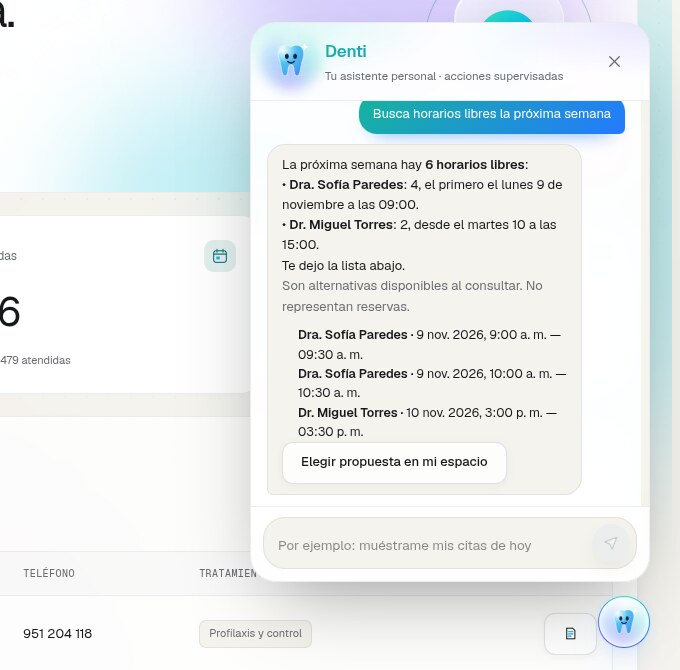
\includegraphics[width=\linewidth]{capturas/m17_denti}}%
  \pgfmathsetmacro\sdpx{\wd\sdimgbox/680}%
  \begin{scope}[x=\sdpx pt,y=-\sdpx pt]
  \node[anchor=north west,inner sep=0pt] (img) at (0,0) {\usebox\sdimgbox};
  \zona{1}{252}{23}{398}{77}
  \zonad{2}{359}{98}{266}{36}
  \zona{3}{267}{144}{315}{180}
  \zona{4}{282}{325}{290}{110}
  \zona{5}{282}{442}{224}{42}
  \zona{6}{263}{518}{374}{50}
  \zonad{7}{598}{596}{52}{52}
  \draw[sdline,line width=0.7pt,rounded corners=3pt] (img.south west) rectangle (img.north east);
  \end{scope}
\end{tikzpicture}
\end{minipage}\hfill
\begin{minipage}[c]{0.46\linewidth}
\small
\begin{list}{}{\leftmargin=2em\labelwidth=1.5em\labelsep=0.5em\itemsep=0.5em}
  \li{1}{Cabecera} Denti y el botón para cerrar.
  \li{2}{Tu instrucción} Lo que escribiste.
  \li{3}{Respuesta} Redactada por el asistente a partir de datos reales.
  \li{4}{Resultados} Horarios o citas encontrados, por profesional.
  \li{5}{Acción sugerida} Lleva la propuesta a Mi espacio para confirmarla.
  \li{6}{Campo de texto} \tecla{Enter} envía.
  \li{7}{Botón flotante} Abre o cierra el panel.
\end{list}
\end{minipage}
\caption{Denti respondiendo una búsqueda de horarios}\label{fig:m17_denti}
\end{figure}

\subsection{Qué puedes pedirle}

\begin{table}[H]
\centering\small
\caption{Ejemplos de instrucciones}\label{tab:denti}
\begin{tabularx}{\linewidth}{@{}P{6.4cm}L@{}}
\toprule
\textbf{Escribe} & \textbf{Denti} \\
\midrule
«¿Qué citas tengo hoy?», «¿y el viernes?» & Lista las citas del día, recordando la conversación. \\
«¿Cuántas citas siguen pendientes esta semana?» & Cuenta y resume por estado. \\
«Busca horarios libres la próxima semana» & Consulta la disponibilidad de cada profesional. \\
«Huecos de la Dra. Paredes el lunes» & Reconoce al profesional por su nombre, con o sin título. \\
«¿Cuántos pacientes tenemos?» & Devuelve el total registrado. \\
«Cancela las citas de mañana de la Dra. Paredes» & Prepara la cancelación y la deja para que la confirmes. \\
\bottomrule
\end{tabularx}
\end{table}

\begin{sdpermiso}
Denti trabaja con tu sesión: a un odontólogo le responde siempre sobre su propia agenda y nunca le pregunta por otro profesional.
\end{sdpermiso}

\begin{sdaviso}[Límites del asistente]
Denti no modifica nada por su cuenta: una cancelación es solo una propuesta hasta que la confirmas. Al modelo de lenguaje no se le envían DNI, teléfonos ni identificadores internos. Revisa siempre sus respuestas antes de tomar decisiones clínicas.
\end{sdaviso}

% =====================================================================
\capitulo{Administración de la clínica}\label{sec:equipo}
% =====================================================================

\acceso{s}{n}{n}

\subsection{Equipo y plan}

\begin{pantalla}{m13_equipo}{1440}{Equipo y plan}
  \zonad{1}{1229}{177}{169}{42}
  \zona{2}{283}{261}{1115}{118}
  \zona{3}{960}{292}{138}{50}
  \zonad{4}{1222}{298}{151}{42}
  \zona{5}{283}{427}{364}{75}
  \zona{6}{876}{450}{84}{26}
  \zonad{7}{971}{445}{38}{38}
\end{pantalla}

\begin{leyenda}
  \li{1}{Agregar miembro} Crea un acceso para el equipo.
  \li{2}{Plan actual} Nombre, condiciones y precio mensual.
  \li{3}{Usuarios en uso} Un punto por usuario permitido.
  \li{4}{Gestionar plan} Cambio de plan.
  \li{5}{Titular} La cuenta responsable; no se puede eliminar.
  \li{6}{Rol} Odontólogo o Recepción.
  \li{7}{Eliminar} Retira el acceso de forma segura.
\end{leyenda}

\begin{table}[H]
\centering\small
\caption{Planes de la clínica}\label{tab:planes}
\begin{tabularx}{\linewidth}{@{}P{2.2cm}C{2.2cm}C{2.4cm}L@{}}
\toprule
\textbf{Plan} & \textbf{Usuarios} & \textbf{Precio} & \textbf{Incluye} \\
\midrule
Básico & Hasta 3 & S/~70 al mes & Panel completo, asistente Denti y menú automático de WhatsApp. \\
Pro & Hasta 8 & S/~100 al mes & Todo lo anterior y respuestas con IA a los pacientes por WhatsApp. \\
\bottomrule
\end{tabularx}
\end{table}

\begin{pasos}
  \paso Pulsa \boton{Agregar miembro} \marca{1}.
  \paso Completa \campo{Nombre completo}, \campo{Correo electrónico}, \campo{Especialidad / Rol en clínica} y una \campo{Contraseña inicial}.
  \paso Pulsa \boton{Crear acceso} y entrega los datos a la persona por un canal privado, pidiéndole que cambie la contraseña al entrar.
\end{pasos}
\resultado{Aparece el aviso «Miembro agregado» y su tarjeta se suma al equipo.}

\begin{sdpeligro}[Retirar un acceso]
\boton{Eliminar} \marca{7} retira el acceso de inmediato. Antes, el sistema permite reasignar sus pacientes y citas a otro profesional para que ningún paciente quede sin responsable. Cuando se alcanza el límite del plan, \boton{Agregar miembro} se desactiva.
\end{sdpeligro}

\needspace{0.55\textheight}
\subsection{Preferencias}

\begin{pantalla}{m14b_preferencias}{1440}{Identidad del consultorio}
  \zona{1}{288}{267}{279}{310}
  \zona{2}{583}{267}{819}{300}
  \zonad{3}{1128}{568}{258}{46}
  \zona{4}{288}{669}{1115}{138}
  \zonad{5}{1212}{715}{171}{46}
\end{pantalla}

\begin{leyenda}
  \li{1}{Logotipo} PNG, JPG, WEBP o SVG de hasta 2~MB.
  \li{2}{Datos de contacto} Nombre del consultorio (obligatorio), dirección, teléfono y correo.
  \li{3}{Descartar y Guardar cambios} Se activan al modificar algo.
  \li{4}{Horario de atención} El que comparte el bot con los pacientes.
  \li{5}{Configurar horario} Lleva a la configuración de WhatsApp.
\end{leyenda}

Debajo de estos bloques está el tarifario, descrito en el \cref{sec:tarifario}.

% =====================================================================
\capitulo{Contraseña y acceso}\label{sec:cuenta}
% =====================================================================

\acceso{s}{s}{s}

\begin{pantalla}{m15_cuenta}{1440}{Cambio de contraseña}
  \zonad{1}{1197}{152}{168}{128}
  \zona{2}{311}{464}{600}{48}
  \pin{3}{885}{457}
  \zona{4}{311}{579}{600}{80}
  \zona{5}{311}{699}{600}{48}
  \zonad{6}{988}{436}{380}{250}
  \zona{7}{311}{765}{179}{42}
\end{pantalla}

\begin{leyenda}
  \li{1}{Usuario y rol} Con qué cuenta y perfil estás conectado.
  \li{2}{Contraseña actual} Necesaria para confirmar que eres tú.
  \li{3}{Mostrar} Muestra u oculta lo escrito.
  \li{4}{Nueva contraseña} Con su medidor de seguridad.
  \li{5}{Confirmación} Debe coincidir con la nueva.
  \li{6}{Lista de comprobación} Cada requisito se marca al cumplirse.
  \li{7}{Actualizar contraseña} Se activa al cumplir todos los requisitos.
\end{leyenda}

La nueva contraseña debe tener \textbf{al menos 12 caracteres}, mayúsculas y minúsculas, al menos un número y un símbolo, y ser distinta de la actual.

\begin{sdconsejo}
Una frase de varias palabras con números y símbolos es más fácil de recordar y más difícil de adivinar. No la reutilices en otros servicios.
\end{sdconsejo}

% =====================================================================
\capitulo{Consola de plataforma}\label{sec:plataforma}
% =====================================================================

\soloplataforma

Al iniciar sesión como administrador de plataforma se abre la consola general, desde la que se gestionan todas las clínicas.

\begin{pantalla}{m20_admin}{1440}{Resumen de negocio de la plataforma}
  \zona{1}{14}{120}{220}{580}
  \zona{2}{319}{314}{304}{42}
  \zona{3}{281}{417}{1118}{178}
  \zona{4}{281}{647}{546}{253}
  \zonad{5}{1219}{22}{180}{40}
  \zona{6}{14}{830}{220}{60}
\end{pantalla}

\begin{leyenda}
  \li{1}{Menú de la consola} General, Facturación y negocio, Operaciones y Mi cuenta.
  \li{2}{Accesos directos} \boton{Explorar clínicas} y \boton{Nueva clínica}.
  \li{3}{Indicadores} Clínicas registradas, activas y suspendidas.
  \li{4}{Distribución} Clínicas activas por plan.
  \li{5}{Fecha y tema} Estado del sistema y cambio de tema.
  \li{6}{Cuenta} Usuario conectado y cierre de sesión.
\end{leyenda}

\begin{table}[H]
\centering\small
\caption{Secciones de la consola}\label{tab:consola}
\begin{tabularx}{\linewidth}{@{}P{4.2cm}L@{}}
\toprule
\textbf{Sección} & \textbf{Uso} \\
\midrule
Dashboard & Indicadores globales de la red de clínicas. \\
Clínicas dentales & Directorio con búsqueda, filtros por estado y alta de clínicas. \\
Suscripciones & Plan asignado a cada clínica y tarifa mensual. \\
Facturas y pagos & Historial de cobros: factura, clínica, fecha, monto, medio y estado. \\
Planes comerciales & Condiciones de los planes Básico y Pro. \\
Operaciones y auditoría & Registro de las acciones administrativas. \\
Configuración global & Ajustes generales de la plataforma. \\
\bottomrule
\end{tabularx}
\end{table}

\needspace{0.55\textheight}
\subsection{Directorio de clínicas}

\begin{pantalla}{m21_clinicas}{1440}{Gestión de clínicas}
  \zonad{1}{1262}{153}{138}{42}
  \zona{2}{281}{255}{1118}{141}
  \zona{3}{307}{518}{743}{44}
  \zonad{4}{1068}{518}{305}{44}
  \zona{5}{307}{683}{1066}{79}
  \zona{6}{1149}{701}{127}{42}
  \zonad{7}{1284}{701}{48}{42}
\end{pantalla}

\begin{leyenda}
  \li{1}{Nueva clínica} Alta de una clínica y de su administrador.
  \li{2}{Indicadores} Registradas, activas y suspendidas.
  \li{3}{Buscar clínica} Por nombre, contacto o dirección.
  \li{4}{Filtro} Todas, activas o suspendidas.
  \li{5}{Fila} Clínica, contacto, plan y estado.
  \li{6}{Administrar} Abre el expediente de la clínica.
  \li{7}{Suspender o reactivar} Cambia el acceso sin borrar datos.
\end{leyenda}

\begin{pasos}
  \paso Pulsa \boton{Nueva clínica} \marca{1}.
  \paso Escribe el nombre de la clínica, el del responsable, el correo de acceso del administrador, la dirección y un teléfono de 9 dígitos.
  \paso Elige el plan (Básico o Pro) y, si lo tienes, sube el logotipo.
  \paso Confirma. El sistema crea la clínica y la cuenta de su administrador y muestra una \textbf{contraseña temporal una sola vez}.
\end{pasos}

\begin{sdaviso}
Copia la contraseña temporal en ese momento y entrégala por un canal seguro: no vuelve a mostrarse.
\end{sdaviso}

\needspace{0.55\textheight}
\subsection{Expediente de una clínica}

\begin{pantalla}{m22_ficha_clinica}{1440}{Expediente de una clínica}
  \zona{1}{24}{33}{180}{36}
  \zona{2}{14}{245}{220}{200}
  \zona{3}{399}{170}{240}{112}
  \zonad{4}{1072}{206}{309}{42}
  \zona{5}{281}{419}{550}{413}
  \zona{6}{883}{764}{498}{42}
  \zonad{7}{1293}{19}{115}{42}
\end{pantalla}

\begin{leyenda}
  \li{1}{Volver} Regresa a la consola.
  \li{2}{Pestañas} Resumen, Equipo, Suscripción y Auditoría.
  \li{3}{Estado y plan} Activa o suspendida, plan asignado.
  \li{4}{Acciones} \boton{Editar clínica} y \boton{Suspender acceso}.
  \li{5}{Datos de la clínica} Registro y contacto.
  \li{6}{Restablecer contraseña} Del administrador de la clínica.
  \li{7}{Directorio} Vuelve a la lista de clínicas.
\end{leyenda}

\begin{sdnota}
Desde el expediente también se exportan los datos de la clínica (pacientes, citas, inventario, transacciones y personal) en JSON o CSV. La suspensión no elimina datos y puede revertirse en cualquier momento.
\end{sdnota}

% =====================================================================
\capitulo{Un caso completo: primera consulta}\label{sec:ejemplo}
% =====================================================================

Este recorrido une los módulos en el orden en que se usan en la práctica.

\begin{figure}[H]
\centering
\begin{tikzpicture}[font=\sffamily\scriptsize,
  st/.style={draw=sdline,fill=white,rounded corners=4pt,minimum width=2.35cm,minimum height=1.25cm,align=center,blur shadow={shadow blur steps=4,shadow opacity=20}},
  ar/.style={-{Stealth[length=5pt]},sdteal,line width=0.9pt}]
  \node[st] (a) {\textcolor{sdteal}{\faIcon{user-plus}}\\[2pt]\textbf{Registro}\\Recepción};
  \node[st,right=0.45cm of a] (b) {\textcolor{sdteal}{\faIcon{calendar-plus}}\\[2pt]\textbf{Reserva}\\Recepción};
  \node[st,right=0.45cm of b] (c) {\textcolor{sdteal}{\faIcon{check-circle}}\\[2pt]\textbf{Confirmación}\\Mi espacio};
  \node[st,right=0.45cm of c] (d) {\textcolor{sdteal}{\faIcon{tooth}}\\[2pt]\textbf{Examen}\\Odontólogo};
  \node[st,right=0.45cm of d] (e) {\textcolor{sdteal}{\faIcon{file-invoice-dollar}}\\[2pt]\textbf{Cotización}\\Odontólogo};
  \node[st,right=0.45cm of e] (f) {\textcolor{sdteal}{\faIcon{cash-register}}\\[2pt]\textbf{Cobro}\\Administración};
  \foreach \x/\y in {a/b,b/c,c/d,d/e,e/f}{\draw[ar] (\x) -- (\y);}
\end{tikzpicture}
\caption{Flujo de una primera consulta}\label{fig:flujo}
\end{figure}

\begin{sdpaso}{1. Registro · Recepción}
En \ruta{Pacientes} pulsa \boton{Nuevo paciente} y registra a «Valeria Quispe» con su teléfono; en alergias escribe «Ninguna».
\end{sdpaso}
\begin{sdpaso}{2. Reserva · Recepción}
Desde su ficha pulsa \boton{Agendar cita}, elige a la Dra. Paredes, el jueves a las 10:30 y el motivo «Consulta / Diagnóstico». La cita queda \estado{sdamber}{Pendiente}.
\end{sdpaso}
\begin{sdpaso}{3. Confirmación}
La paciente confirma por WhatsApp. En la agenda abre la cita, pulsa \boton{Revisar en Mi espacio} y confirma. La tarjeta pasa a \estado{sdteal}{Confirmada}.
\end{sdpaso}
\begin{sdpaso}{4. Examen · Odontólogo}
En \ruta{Odontograma} elige a la paciente, pulsa \tecla{1} y marca en rojo una caries oclusal y mesial en la 16; con \tecla{2} y \boton{Buen estado}, la restauración existente de la 26. Escribe «Control en 6 meses» y pulsa \boton{Guardar odontograma}.
\end{sdpaso}
\begin{sdpaso}{5. Cotización · Odontólogo}
La cotización propone resina más una cara adicional en la 16: S/~110. Añade \textit{Profilaxis y destartraje}, pulsa \boton{Imprimir} para entregársela y \boton{Guardar cotización}.
\end{sdpaso}
\begin{sdpaso}{6. Cobro · Administración}
En \ruta{Caja e ingresos} pulsa \boton{Registrar ingreso}: S/~50, «Consulta y diagnóstico», método Yape, paciente Valeria Quispe.
\end{sdpaso}

% =====================================================================
\capitulo{Solución de problemas}\label{sec:problemas}
% =====================================================================

\begin{longtable}{@{}P{4.6cm}P{4.4cm}P{5.6cm}@{}}
\caption{Problemas frecuentes, causa y solución}\label{tab:problemas}\\
\toprule
\textbf{Síntoma} & \textbf{Causa probable} & \textbf{Qué hacer} \\
\midrule\endfirsthead
\toprule
\textbf{Síntoma} & \textbf{Causa probable} & \textbf{Qué hacer} \\
\midrule\endhead
\small No puedo iniciar sesión. & \small Correo o contraseña incorrectos, o clínica suspendida. & \small Revisa mayúsculas y espacios; usa \textit{¿Olvidaste tu contraseña?}. Si persiste, consulta a la administración. \\
\small La sesión se cerró sola. & \small La sesión caduca por seguridad. & \small Vuelve a entrar; lo guardado no se pierde. \\
\small No veo una sección del menú. & \small Tu perfil no tiene acceso (\cref{tab:matriz}). & \small Pide a la administración que revise tu rol. \\
\small No aparecen horarios al reservar. & \small El profesional no atiende ese día o está ocupado. & \small Prueba otra fecha u otro profesional. \\
\small «Horario pasado». & \small La hora elegida ya transcurrió. & \small Elige un horario futuro. \\
\small «No se confirmó el cambio». & \small La conexión se interrumpió antes de la respuesta. & \small Actualiza la vista y comprueba si el cambio se guardó antes de repetirlo. \\
\small La cotización está en cero. & \small No hay marcas en rojo o todas se desmarcaron. & \small Registra hallazgos con \boton{Mal estado} o vuelve a marcar las líneas. \\
\small La vista 3D no se muestra. & \small El navegador tiene desactivada la aceleración gráfica. & \small Actívala o usa la vista 2D, que contiene el mismo registro. \\
\small No puedo agregar más miembros. & \small Se alcanzó el límite del plan. & \small Retira un acceso o cambia al plan Pro. \\
\small Un mensaje queda «Envío por confirmar». & \small WhatsApp aún no respondió. & \small Espera la confirmación; no lo reenvíes. \\
\small Denti responde que no encontró datos. & \small No existen en el periodo consultado o tu perfil no los ve. & \small Amplía el periodo o reformula la pregunta. \\
\bottomrule
\end{longtable}

\subsection{Preguntas frecuentes}

\paragraph{¿Se pierde algo si cierro el navegador sin guardar el odontograma?} Sí: los cambios no guardados se descartan. Por eso el sistema avisa al intentar salir con cambios pendientes.

\paragraph{¿Puedo recuperar una versión anterior del odontograma?} Cada guardado queda en el \textit{Historial} con su fecha y autor, y puede consultarse en cualquier momento.

\paragraph{¿Otra clínica puede ver a mis pacientes?} No. Cada clínica tiene sus datos aislados en la base de datos, con reglas que se aplican a cada consulta.

\paragraph{¿El paciente recibe la cotización automáticamente?} No. Se imprime o se guarda como PDF y la entregas tú; la copia guardada queda en su ficha.

\paragraph{¿Denti puede equivocarse?} Denti consulta datos reales en lugar de inventarlos, pero su redacción debe revisarse. Las acciones que cambian datos siempre requieren tu confirmación.

% =====================================================================
\capitulo{Referencia rápida}\label{sec:referencia}
% =====================================================================

\subsection{Atajos de teclado}

\begin{table}[H]
\centering\small
\caption{Atajos de teclado}\label{tab:atajos}
\begin{tabularx}{\linewidth}{@{}P{4.4cm}L P{3cm}@{}}
\toprule
\textbf{Atajo} & \textbf{Acción} & \textbf{Dónde} \\
\midrule
\tecla{Ctrl}\,+\,\tecla{K} & Abrir o cerrar la búsqueda rápida & Todo el sistema \\
\tecla{$\uparrow$}\,\tecla{$\downarrow$}\ \tecla{Enter}\ \tecla{Esc} & Moverse, abrir y cerrar & Búsqueda rápida \\
\tecla{1} … \tecla{9} & Elegir herramienta & Odontograma \\
\tecla{0} & Herramienta Borrar & Odontograma \\
\tecla{$\leftarrow$}\,\tecla{$\rightarrow$} & Pieza anterior o siguiente & Odontograma \\
\tecla{Ctrl}\,+\,\tecla{Z} & Deshacer & Odontograma \\
\tecla{Ctrl}\,+\,\tecla{Shift}\,+\,\tecla{Z} & Rehacer & Odontograma \\
\tecla{Enter} & Enviar instrucción & Denti \\
\tecla{Esc} & Cerrar ventanas y paneles & Todo el sistema \\
\bottomrule
\end{tabularx}
\end{table}

\subsection{Glosario}

\begin{description}[font=\sffamily\bfseries\color{sdink},leftmargin=0pt,itemsep=0.3em]
  \item[Arcada] Conjunto de piezas de un maxilar; la vista 3D muestra ambas.
  \item[ceo-d] Índice de dentición temporal: piezas cariadas, con extracción indicada y obturadas.
  \item[CPO-D] Índice de dentición permanente: piezas cariadas, perdidas y obturadas.
  \item[Cotización] Presupuesto aproximado calculado desde los hallazgos y el tarifario.
  \item[Dentición mixta] Coexistencia de piezas temporales y permanentes.
  \item[FDI] Numeración dental internacional de dos dígitos: cuadrante y posición.
  \item[Hallazgo] Condición que requiere atención; se marca en rojo.
  \item[Mi espacio] Sección donde se revisan y confirman los cambios antes de aplicarlos.
  \item[Stock mínimo] Cantidad a partir de la cual un insumo se considera bajo.
  \item[Tarifario] Lista de precios de la clínica que usa la cotización.
\end{description}

\end{document}
